
Raft's log grows during normal operation as it incorporates more client
requests. As it grows larger, it occupies more space and takes more time
to replay. Without some way to compact the log, this will eventually
cause availability problems: servers will either run out of space, or
they will take too long to start. Thus, some form of log compaction is
necessary for any practical system.

The general idea of log compaction is that much of the information in
the log becomes obsolete over time and can be discarded. For example, an
operation that sets $x$ to 2 is obsolete if a later operation sets $x$
to 3. Once log entries have been committed and applied to the
state machine, the intermediate states and operations used to arrive at
the current state are no longer needed, and they can be compacted away.

Unlike the core Raft algorithm and membership changes, different systems
will have different needs when it comes to log compaction. There is no
one-size-fits-all solution to log compaction for a couple of reasons.
First, different systems may choose to trade off simplicity and
performance to varying degrees. Second, the state machine must be
intimately involved in log compaction, and state machines differ
substantially in size and in whether they are based on disk or volatile memory.

\begin{figure*}
\centering
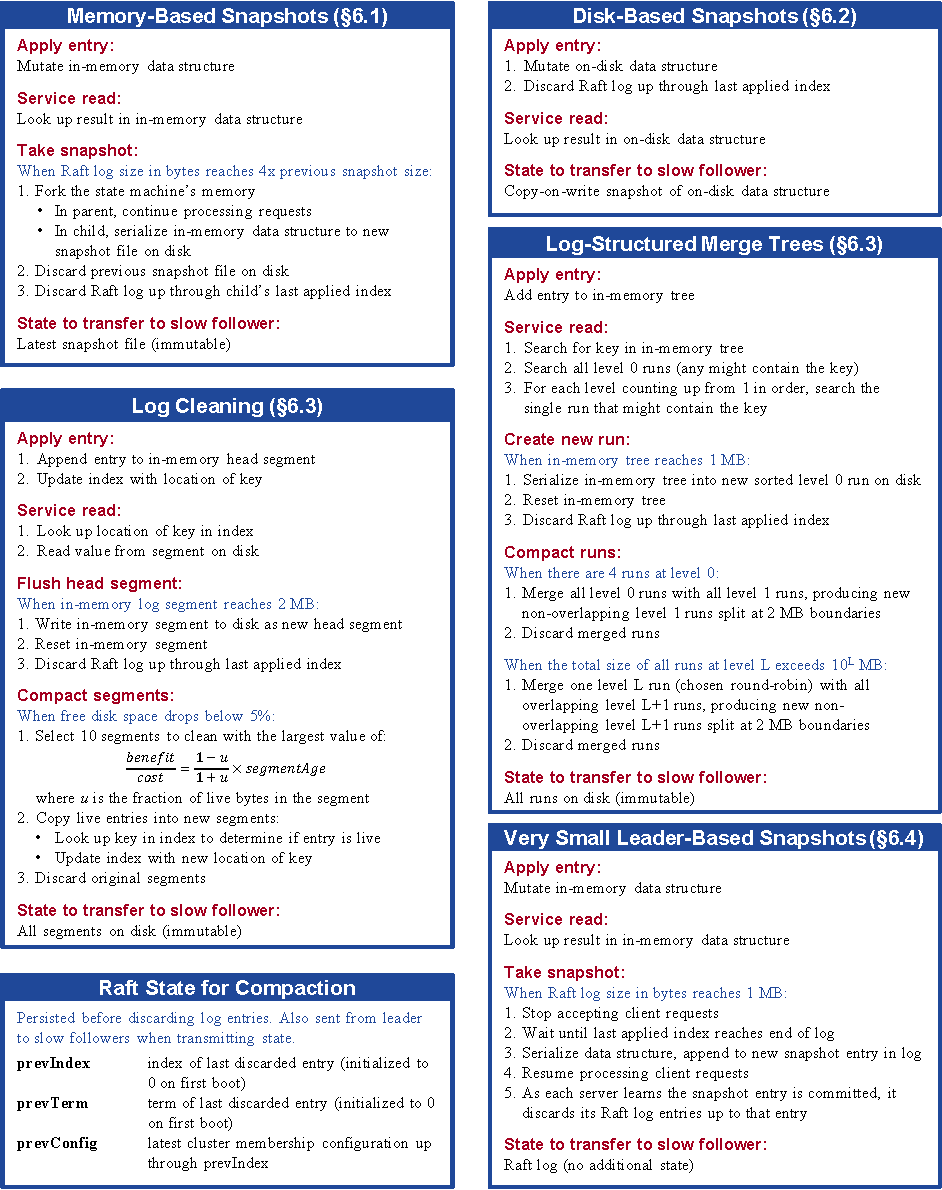
\includegraphics[scale=0.95]{compaction/rules}
\vcaption[summary of approaches]{
The figure shows how various approaches to log compaction can be used in
Raft. Details for log-structured merge trees in the figure are based
on LevelDB~\cite{leveldb:compactions}, and details for log cleaning are
based on RAMCloud~\cite{Rumble:2014}; rules for managing deletions are
omitted.
}
\label{fig:compaction:rules}
\end{figure*}

The goal of this chapter is to discuss a variety of approaches to log
compaction. In each approach, most of the responsibility of log
compaction falls on the state machine, which is in charge of writing the
state to disk and compacting the state. State machines can achieve this
in different ways, which are described throughout the chapter and
summarized in Figure~\ref{fig:compaction:rules}:
%
\begin{itemize}
%
\item
%
Snapshotting for memory-based state machines is conceptually the
simplest approach. In snapshotting, the entire current system state is
written to a \emph{snapshot} on stable storage, then the entire log up
to that point is discarded. Snapshotting is used in
Chubby~\cite{Burrows:2006, Chandra:2007} and ZooKeeper~\cite{Hunt:2010},
and we have implemented snapshotting in LogCabin. Snapshotting is the
approach presented in the most depth in this chapter,
in Section~\ref{compaction:memsnapshot}.
%
\item
%
With disk-based state machines, a recent copy of the system state is
maintained on disk as part of normal operation. Thus, the Raft log can
be discarded as soon as the state machine reflects writes to disk,
and snapshotting is used only when sending consistent disk images to
other servers
(Section~\ref{compaction:disksnapshot}).
%
\item
%
Incremental approaches to log compaction, such as log cleaning and
log-structured merge trees, are presented in
Section~\ref{compaction:incremental}. These approaches write to disk
efficiently, and they utilize resources evenly over time.
%
\item
%
Finally, Section~\ref{compaction:leader} discusses an approach to log
compaction that minimizes the mechanism required by storing snapshots
directly in the log. Though easier to implement, this approach is only
suitable for very small state machines.
%
\end{itemize}
%
LogCabin currently only implements the memory-based snapshotting
approach (it embeds a memory-based state machine).

The various approaches to compaction share several core concepts. First,
instead of centralizing compaction decisions on the leader, each server
compacts the
committed prefix of its log independently. This avoids having the leader
transmit data to followers that already have the data in their logs. It also
helps modularity: most of the complexity of log compaction is
contained within the state machine and does not interact much with Raft
itself. This helps keep overall system complexity to a
minimum: the complexity of Raft adds to, rather than multiplies with,
the complexity of log compaction. Alternative approaches that centralize compaction
responsibilities on a leader are discussed further in
Section~\ref{compaction:leader} (and for very small state machines, a
leader-based approach may be better).

Second, the basic interaction between the state machine and Raft
involves transferring responsibility for a prefix of the log from Raft
to the state machine.
Sooner or later after applying entries, the state machine reflects those
entries to disk in a way that can recover the current system state.
Once it has done so, it tells Raft to discard the corresponding
prefix of the log. 
Before Raft can give up responsibility for the log prefix,
it must save some of its own state describing the log prefix.
Specifically, Raft retains the index and term of the last entry it
discarded; this anchors the rest of the log in place after the state
machine's state and allows the AppendEntries consistency check to
continue to work (it needs the index and term for the entry preceding
the first entry in the log). Raft also retains the latest configuration
from the discarded log prefix in order to support cluster membership
changes.

Third, once Raft has discarded a prefix of the log, the state machine
takes on two new responsibilities. If the server restarts, the state
machine will need to load the state corresponding to the discarded log
entries from disk before it can apply any entries from the Raft log.
In addition, the state machine may need to produce a consistent image of
the state so that it can be sent to a slow follower
(one whose log is far behind the leader's). It is not feasible
to defer compaction  until log entries have been ``fully replicated'' to
every member in the cluster, since a minority of slow followers must not
keep the cluster from being fully available, and new servers can be
added to the cluster at any time. Thus, slow followers or new servers
will occasionally need to receive their initial states over the network.
Raft detects this when the next entry needed in AppendEntries has
already been discarded in the leader's log. In this case, the state
machine must provide a consistent image of the state, which the leader
then sends to the follower.


